\chapter{Contenedor LXC con acceso a GPU y stack CUDA 6.5} \label{cap4}

En este capítulo se describe la configuración del contenedor LXC con acceso directo a ambas GPUs, la instalación del stack \textit{userspace} de NVIDIA dentro del contenedor y la instalación del último toolkit CUDA compatible con las arquitecturas del hardware (CUDA 6.5). El capítulo culmina con la validación del cómputo real mediante \texttt{deviceQuery}.

\section{Objetivo}

Partimos de la situación alcanzada en el capítulo 3: el driver 340.108 está instalado y funcionando en el host vía DKMS, con \texttt{nvidia-smi} operativo y detectando ambas tarjetas. El objetivo ahora es crear un contenedor LXC en Proxmox VE 9 con acceso directo (paso de dispositivos) a ambas GPUs, e instalar dentro de él el stack CUDA 6.5 para validar cómputo real.

La figura \ref{fig:arquitectura} resume la arquitectura del sistema completo en su estado final: el host Proxmox carga el módulo de kernel del driver (único driver del sistema), y el contenedor \texttt{gpu-tfg} accede a las tarjetas mediante \textit{bind mounts} de los \textit{character devices}.

\begin{figure}[htbp]
\centering
% Figura precompilada para reducir el tiempo de compilacion.
% Fuente editable: figuras/capitulo4/arquitectura-sistema.tex
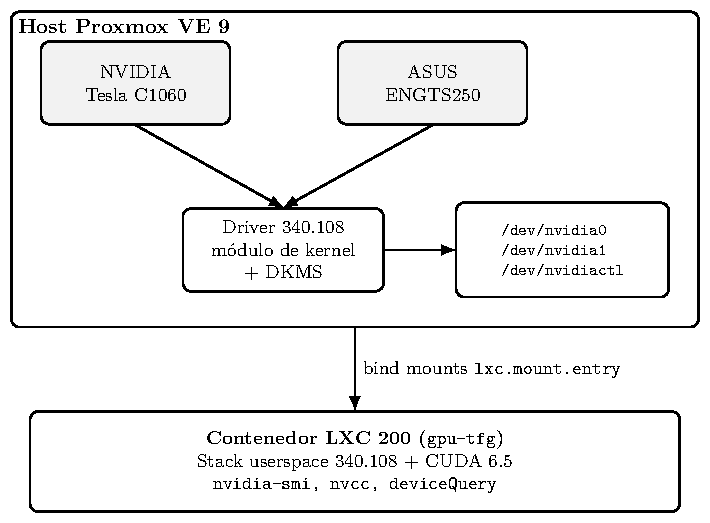
\includegraphics{figuras/capitulo4/arquitectura-sistema}
\caption{Arquitectura del sistema: host Proxmox con el driver, y contenedor LXC con acceso a ambas GPUs}
\label{fig:arquitectura}
\end{figure}

\section{Selección de almacenamiento}

Antes de crear el contenedor se verificó el almacenamiento disponible en Proxmox con \texttt{pvesm status}, que arrojó dos \textit{storages} con usos complementarios (tabla \ref{tab:storage}):

\begin{table}[htbp]
\centering
\begin{tabular}{|l|l|l|}
\hline
\textbf{Storage} & \textbf{Tipo} & \textbf{Uso recomendado} \\
\hline
\texttt{local} & \texttt{dir} & Plantillas (\texttt{vztmpl}), ISOs, backups \\
\hline
\texttt{local-lvm} & \texttt{lvmthin} & Discos de VMs y rootfs de contenedores \\
\hline
\end{tabular}
\caption{Almacenamiento disponible en Proxmox}
\label{tab:storage}
\end{table}

Se decidió usar \texttt{local-lvm} para el \textit{rootfs} del contenedor y \texttt{local} únicamente como origen de la plantilla de sistema.

\section{Obtención de la plantilla de sistema}

La plantilla se obtiene con \texttt{pveam} (administrador de plantillas de contenedores): \texttt{pveam update}, \texttt{pveam available} y \texttt{pveam download}. Una observación importante de esta fase es que el nombre exacto de la plantilla (número de \textit{build} tras \texttt{debian-12-standard\_12.X-1\_amd64.tar.zst}) varía con el tiempo según lo que Proxmox tenga indexado en el momento; debe consultarse siempre con \texttt{pveam available} antes de descargar, en lugar de asumir una versión fija.

\section{Creación del contenedor}

El contenedor se creó con el siguiente comando:

\begin{lstlisting}[style=bash]
pct create 200 local:vztmpl/<plantilla>.tar.zst \
  --hostname gpu-tfg \
  --cores 4 \
  --memory 4096 \
  --rootfs local-lvm:32 \
  --net0 name=eth0,bridge=vmbr0,ip=dhcp \
  --unprivileged 0 \
  --features nesting=1
\end{lstlisting}

Dos decisiones de diseño son relevantes. En primer lugar, se optó deliberadamente por un \textbf{contenedor privilegiado} en lugar de no privilegiado. Los contenedores no privilegiados aplican un remapeo de UID/GID entre el \textit{namespace} del contenedor y el host \cite{lxc_security,lxc_containers_conf}, lo que complica significativamente el acceso a \textit{character devices} como los de NVIDIA (habría que mapear también los grupos propietarios de \texttt{/dev/nvidia*}). Para un entorno experimental como el de este trabajo, la vía privilegiada es la más simple y directa, a costa de un aislamiento de seguridad menor, una decisión razonable dado el contexto puramente experimental del proyecto.

En segundo lugar, \texttt{--features nesting=1} prepara el contenedor por si se requiere anidar otros entornos (Docker, otro LXC) en fases posteriores.

\section{Identificación de los device nodes en el host}

El siguiente paso es identificar los \textit{device nodes} que expone el driver en el host. El resultado relevante de \texttt{cat /proc/devices | grep -i nvidia} es:

\begin{lstlisting}[style=bash]
195 nvidia-frontend
\end{lstlisting}

El \textit{major} 195 corresponde al \textit{frontend} del driver NVIDIA y es el que expone \texttt{/dev/nvidia0}, \texttt{/dev/nvidia1} y \texttt{/dev/nvidiactl}. No aparece ningún \textit{major} para \texttt{nvidia-uvm} porque el módulo \texttt{nvidia-uvm.ko} no se compiló deliberadamente (véase el capítulo 3); por tanto, la configuración del contenedor no incluye el bloque de paso de dispositivo para UVM.

El mapeo de GPUs, confirmado con \texttt{nvidia-smi} en el host, es:

\begin{table}[htbp]
\centering
\begin{tabular}{|l|l|l|}
\hline
\textbf{Device node} & \textbf{GPU} & \textbf{Bus PCI} \\
\hline
\texttt{/dev/nvidia0} & Tesla C1060 & \texttt{0000:01:00.0} \\
\hline
\texttt{/dev/nvidia1} & GeForce GTS 250 (ENGTS250) & \texttt{0000:08:00.0} \\
\hline
\texttt{/dev/nvidiactl} & (control, compartido) & --- \\
\hline
\end{tabular}
\caption{Mapeo de device nodes a GPUs en el host}
\label{tab:devices}
\end{table}

\section{Configuración del paso de dispositivos}

La configuración del contenedor se realiza en \texttt{/etc/pve/lxc/200.conf}, añadiendo el permiso de \textit{cgroup} sobre el \textit{major} del driver y los \textit{bind mounts} de cada dispositivo:

\begin{lstlisting}[style=bash]
lxc.cgroup2.devices.allow: c 195:* rwm
lxc.mount.entry: /dev/nvidia0 dev/nvidia0 none bind,optional,create=file
lxc.mount.entry: /dev/nvidia1 dev/nvidia1 none bind,optional,create=file
lxc.mount.entry: /dev/nvidiactl dev/nvidiactl none bind,optional,create=file
\end{lstlisting}

Esta configuración proporciona acceso a \textbf{ambas GPUs simultáneamente} desde el mismo contenedor. Para un escenario de aislamiento por GPU (un contenedor por tarjeta, de interés para comparativas de rendimiento aisladas), bastaría con omitir el \texttt{lxc.mount.entry} de la GPU no deseada en cada \texttt{.conf} respectivo.

Antes de arrancar el contenedor es necesario comprobar que los nodos existen en el host; si no, se fuerza su creación ejecutando \texttt{nvidia-smi} una vez. Tras el arranque (\texttt{pct start 200}), se confirmó que los tres \textit{device nodes} (\texttt{nvidia0}, \texttt{nvidia1}, \texttt{nvidiactl}) llegan correctamente al \textit{namespace} del contenedor con el mismo \textit{major} 195.

\section{Instalación del stack userspace NVIDIA en el contenedor}

A diferencia del módulo de kernel, que requirió el proceso extenso de parcheo documentado en el capítulo 3, el stack \textit{userspace} (librerías \texttt{libcuda}, \texttt{nvidia-smi}, etc.) es un binario precompilado por NVIDIA y \textbf{no depende de dichos parches}. Por tanto, dentro del contenedor se utiliza el instalador \texttt{.run} oficial sin modificar, únicamente con el flag \texttt{--no-kernel-module} que omite la instalación del módulo de kernel (compartido con el host). Los \textit{prompts} respondidos durante la instalación son idénticos a los del host y por el mismo motivo (entorno sin X11): no instalar las librerías de compatibilidad de 32 bits y no generar configuración X11.

La verificación con \texttt{nvidia-smi} confirma que ambas GPUs son visibles y accesibles desde dentro del contenedor, con la misma versión de driver (340.108) que el host, validando la compatibilidad ABI entre el módulo de kernel (host) y las librerías \textit{userspace} (contenedor).

\section{CUDA Toolkit 6.5}

\subsection{Justificación de la versión}

Las \textit{compute capabilities} de las GPUs del proyecto son 1.3 (Tesla C1060) y 1.1 (GTS 250). El CUDA Toolkit 6.5 es la última versión con soporte para \textit{compute capability} $<$ 2.0 (arquitectura Tesla/GT200); las versiones posteriores del \textit{toolkit} eliminan dicho soporte \cite{nvidia_legacy_gpus}. Por tanto, el toolkit a instalar dentro del contenedor no puede ser superior a CUDA 6.5.

\subsection{Descarga}

La descarga se realiza desde el enlace directo del instalador \cite{cuda_65_archive}, que apunta al fichero \texttt{cuda\_6.5.14\_linux\_64.run}.

\subsection{Primer obstáculo: compilador no soportado}

El instalador rechazó el compilador del sistema:

\begin{lstlisting}[style=bash]
Error: unsupported compiler: 12.2.0. Use --override to override this check.
\end{lstlisting}

CUDA Toolkit 6.5 (2014) declara soporte oficial hasta gcc 4.8.x, mientras que el contenedor, con Debian 12, tiene gcc 12.2.0 por defecto: una diferencia de ocho versiones principales. La solución fue usar el flag \texttt{--override} del instalador para omitir la comprobación. Este obstáculo es el mismo tipo de obsolescencia de software \textit{legacy} documentada para el driver de kernel en el capítulo 3.

\subsection{Segundo obstáculo: fallo silencioso del meta-instalador}

Ejecutar el meta-instalador en modo silencioso con \texttt{--override} completó ``sin errores visibles'', pero el toolkit no quedó instalado (\texttt{/usr/local/cuda-6.5/bin/} vacío salvo el script de desinstalación). El log (\texttt{/tmp/cuda\_install\_*.log}) reveló la causa real:

\begin{lstlisting}[style=bash]
Can't locate InstallUtils.pm in @INC (...) at ./install-linux.pl line 6.
BEGIN failed--compilation aborted at ./install-linux.pl line 6.
\end{lstlisting}

El diagnóstico es interesante: el \texttt{.run} de CUDA 6.5 es en realidad un \textbf{meta-instalador} que empaqueta tres subinstaladores independientes (driver, toolkit y \textit{samples}), cada uno también autoextraíble (formato \textit{makeself}). El script Perl \texttt{install-linux.pl} del subinstalador del toolkit no resolvía correctamente la ruta de su propio módulo auxiliar \texttt{InstallUtils.pm} al ejecutarse a través del flujo normal de autoextracción/autoejecución encadenada (extracción a directorio temporal autodestruible, con \texttt{@INC} de Perl no ajustado a esa ruta).

\subsection{Solución: extracción manual en dos niveles}

La solución consistió en extraer manualmente por capas. En el \textbf{nivel 1} se extrajeron los tres subinstaladores del meta-instalador con la opción \texttt{--extract} del propio \texttt{.run}. En el \textbf{nivel 2} se extrajo el sub-instalador del toolkit a una ruta persistente, usando las opciones propias de \textit{makeself}:

\begin{lstlisting}[style=bash]
./cuda-linux64-rel-6.5.14-18749181.run --keep --target ~/cuda-toolkit-extracted --noexec
\end{lstlisting}

\texttt{--noexec} evita la ejecución automática tras extraer; \texttt{--keep --target} fuerza que el contenido quede en una ruta fija en vez de un \texttt{/tmp} aleatorio autodestruible. Con el contenido a la vista, el instalador Perl pudo ejecutarse manualmente forzando la ruta de búsqueda de módulos: \texttt{perl -I. ./install-linux.pl -noprompt -prefix=/usr/local/cuda-6.5}. El flag \texttt{-I.} añade explícitamente el directorio actual a \texttt{@INC}, resolviendo la incapacidad del script original para localizar su propio módulo auxiliar.

\subsection{Instalación de los samples}

El subinstalador de \textit{samples} presenta la misma arquitectura (y el mismo problema potencial), por lo que se aplicó el mismo patrón de extracción manual. El intento con el script auxiliar \texttt{cuda-install-samples-6.5.sh} falló por asumir una estructura de directorios distinta a la real del paquete (\texttt{../samples/*} en vez de \texttt{./cuda-samples/*}). La solución adoptada fue una copia manual directa del árbol, evitando depender de scripts frágiles para un paso que es, en esencia, una simple copia de directorios.

\subsection{Configuración del entorno}

Por último se añadieron al \texttt{.bashrc} las variables de entorno \texttt{PATH} y \texttt{LD\_LIBRARY\_PATH} apuntando a \texttt{/usr/local/cuda-6.5}, quedando \texttt{nvcc} operativo y reportando \texttt{release 6.5, V6.5.14}.

\section{Validación de cómputo real: \texttt{deviceQuery}}

A diferencia de \texttt{nvidia-smi} (que solo confirma \emph{detección} de hardware), el ejemplo \texttt{deviceQuery} del SDK de CUDA compila y ejecuta código real contra el \textit{runtime} CUDA, constituyendo la prueba definitiva de que el cómputo GPU funciona de extremo a extremo dentro del contenedor. Conviene recordar aquí la distinción entre las dos APIs de CUDA: la \textit{Driver API} da acceso directo al contexto, a los módulos y a los módulos binarios, mientras que la \textit{Runtime API} se implementa por encima de la anterior y aporta inicialización implícita, gestión de contexto y de módulos a cambio de un menor control \cite{nvidia_driver_vs_runtime,so_cuda_driver_runtime}. El uso del \textit{runtime} es precisamente lo que explica el campo \texttt{CUDA Driver = CUDART} de la salida del benchmark, y es también la razón por la que la compatibilidad ABI entre el módulo de kernel del host y las librerías del contenedor solo se puede validar ejecutando código real, y no consultando únicamente \texttt{nvidia-smi}. El resultado obtenido fue:

\begin{lstlisting}[style=bash]
Detected 2 CUDA Capable device(s)
deviceQuery, CUDA Driver = CUDART, CUDA Driver Version = 6.5, CUDA Runtime Version = 6.5,
NumDevs = 2, Device0 = Tesla C1060, Device1 = GeForce GTS 250
Result = PASS
\end{lstlisting}

Con \texttt{Result = PASS}, queda validado el cómputo CUDA real de extremo a extremo dentro del contenedor LXC, cerrando el objetivo técnico principal de esta fase del trabajo. La salida completa de \texttt{deviceQuery} para ambas tarjetas se proporciona como material complementario (apéndice~\ref{ape:host}).

Como se adelantó en el capítulo 3, la salida de \texttt{deviceQuery} confirmó también, con datos reales y no solo con el argumento teórico de \textit{compute capability}, que ambas GPUs reportan \texttt{Device supports Unified Addressing (UVA): No}, validando la decisión de no compilar el módulo \texttt{nvidia-uvm.ko} en el host: el hardware no soporta esa característica independientemente del software instalado.

\section{Valoración de la fase}

Desde el punto de vista cualitativo, esta fase aporta dos resultados de interés para el objetivo general del trabajo. En primer lugar, demuestra que \textbf{el paso de dispositivos a contenedores es notablemente más simple que la vía de las máquinas virtuales}: toda la complejidad de la fase anterior (IOMMU, grupos, resets) desaparece, y el coste se traslada a la instalación del driver en el host, que ya estaba resuelta en el capítulo 3. En segundo lugar, la experiencia con CUDA 6.5 confirma un patrón recurrente en este trabajo: \textbf{los instaladores antiguos fallan silenciosamente ante entornos modernos}, y la única vía robusta es la extracción y ejecución manual por capas. Este patrón, que se repetirá en el capítulo 5 con el front-end de \texttt{nvcc}, es una lección metodológica transferible a cualquier proyecto que reutilice software \textit{legacy}: los flujos automáticos de instalación de hace diez años no pueden darse por supuestos.

\section{Notas operativas}

Durante el proceso se generaron accidentalmente contenedores duplicados bajo el mismo VMID original (200) al reejecutarse \texttt{pct create} sin percatarse de que el contenedor ya existía, dejando el disco original (\texttt{vm-200-disk-0}, 32 GB, con toda la instalación funcional) huérfano pero intacto en el storage \texttt{local-lvm}. Se recuperó reasignando dicho disco a un nuevo VMID (202), que es el contenedor definitivo y operativo a partir de este punto del proyecto.

La lección documentable para este tipo de entornos es doble. Primero, antes de relanzar un comando \texttt{pct create} sobre un VMID ya en uso, hay que verificar siempre su estado con \texttt{pct list} y \texttt{pct config <vmid>}: Proxmox no impide crear un nuevo disco bajo un ID ya existente si la invocación difiere ligeramente (por ejemplo, en el tamaño de \texttt{--rootfs}), lo que puede dejar volúmenes huérfanos y generar confusión sobre cuál es el entorno de trabajo activo. Segundo, el comando \texttt{hostnamectl set-hostname} debe ejecutarse siempre \emph{dentro} del contenedor o VM cuyo nombre se quiere cambiar, nunca en el host de Proxmox: cambiar el \textit{hostname} del propio nodo rompe temporalmente la resolución de rutas de \texttt{pmxcfs} (\texttt{/etc/pve/nodes/<hostname>/...}), dejando inaccesibles todas las configuraciones de VMs y contenedores hasta revertirlo.

Con el entorno de cómputo plenamente operativo, el siguiente capítulo aborda la experimentación: benchmarks de rendimiento, contención concurrente y análisis de limitaciones del hardware.

